\documentclass[nocopyrightspace]{acm_proc_article-sp}
\usepackage{url}
\usepackage{subfig}
\usepackage{color,soul}
\usepackage{enumitem}

\definecolor{lightgray}{rgb}{0.95, 0.95, 0.95}
\definecolor{darkgray}{rgb}{0.4, 0.4, 0.4}
\definecolor{editorGray}{rgb}{0.95, 0.95, 0.95}
\definecolor{editorOcher}{rgb}{1, 0.5, 0}
\definecolor{editorGreen}{rgb}{0, 0.5, 0}
\definecolor{orange}{rgb}{1,0.45,0.13}      
\definecolor{olive}{rgb}{0.17,0.59,0.20}
\definecolor{brown}{rgb}{0.69,0.31,0.31}
\definecolor{purple}{rgb}{0.38,0.18,0.81}
\definecolor{lightblue}{rgb}{0.1,0.57,0.7}
\definecolor{lightred}{rgb}{1,0.4,0.5}

\usepackage{upquote}
\usepackage{listings}

% JavaScript
\lstdefinelanguage{JavaScript}{
    morekeywords={typeof, new, true, false, catch, function, return, null, catch, switch, var, if, in, while, do, else, case, break},
    morecomment=[s]{/*}{*/},
    morecomment=[l]//,
    morestring=[b]",
    morestring=[b]'
}

\lstdefinestyle{pystyle} {%
    language=python,
    literate=%
    *{0}{{{\color{lightred}0}}}1
    {1}{{{\color{lightred}1}}}1
    {2}{{{\color{lightred}2}}}1
    {3}{{{\color{lightred}3}}}1
    {4}{{{\color{lightred}4}}}1
    {5}{{{\color{lightred}5}}}1
    {6}{{{\color{lightred}6}}}1
    {7}{{{\color{lightred}7}}}1
    {8}{{{\color{lightred}8}}}1
    {9}{{{\color{lightred}9}}}1,
    basicstyle=\footnotesize\ttfamily, % Standardschrift
    numbers=none,               % Ort der Zeilennummern
    %numberstyle=\tiny,          % Stil der Zeilennummern
    %stepnumber=2,               % Abstand zwischen den Zeilennummern
    numbersep=5pt,              % Abstand der Nummern zum Text
    tabsize=4,                  % Groesse von Tabs
    extendedchars=true,         %
    breaklines=true,            % Zeilen werden Umgebrochen
    keywordstyle=\color{blue}\bfseries,
    commentstyle=\color{brown}\itshape,
    stringstyle=\color{editorOcher}\ttfamily, % Farbe der String
    showspaces=false,           % Leerzeichen anzeigen ?
    showtabs=false,
    xleftmargin={0cm},
    showstringspaces=false,      % Leerzeichen in Strings anzeigen ?
}

\lstdefinestyle{htmlcssjs} {%
    % General design
    %  backgroundcolor=\color{editorGray},
    basicstyle={\footnotesize\ttfamily},   
    % line-numbers
    xleftmargin={0cm},
    numbers=none, 
    % Code design
    identifierstyle=\color{black},
    keywordstyle=\color{blue}\bfseries,
    ndkeywordstyle=\color{editorGreen}\bfseries,
    stringstyle=\color{editorOcher}\ttfamily,
    commentstyle=\color{brown}\ttfamily,
    % Code
    language=JavaScript,
    alsodigit={.:;},  
    tabsize=2,
    showtabs=false,
    showspaces=false,
    showstringspaces=false,
    extendedchars=true,
    breaklines=true
}

\lstdefinestyle{py} {%
    language=python,
    literate=%
    *{0}{{{\color{lightred}0}}}1
    {1}{{{\color{lightred}1}}}1
    {2}{{{\color{lightred}2}}}1
    {3}{{{\color{lightred}3}}}1
    {4}{{{\color{lightred}4}}}1
    {5}{{{\color{lightred}5}}}1
    {6}{{{\color{lightred}6}}}1
    {7}{{{\color{lightred}7}}}1
    {8}{{{\color{lightred}8}}}1
    {9}{{{\color{lightred}9}}}1,
    basicstyle=\footnotesize\ttfamily, % Standardschrift
    numbers=left,               % Ort der Zeilennummern
    %numberstyle=\tiny,          % Stil der Zeilennummern
    %stepnumber=2,               % Abstand zwischen den Zeilennummern
    numbersep=5pt,              % Abstand der Nummern zum Text
    tabsize=4,                  % Groesse von Tabs
    extendedchars=true,         %
    breaklines=true,            % Zeilen werden Umgebrochen
    keywordstyle=\color{blue}\bfseries,
    frame=b,
    commentstyle=\color{brown}\itshape,
    stringstyle=\color{editorOcher}\ttfamily, % Farbe der String
    showspaces=false,           % Leerzeichen anzeigen ?
    showtabs=false,             % Tabs anzeigen ?
    xleftmargin=17pt,
    framexleftmargin=17pt,
    framexrightmargin=5pt,
    framexbottommargin=4pt,
    %backgroundcolor=\color{lightgray},
    showstringspaces=false,      % Leerzeichen in Strings anzeigen ?
}


\lstdefinestyle{sql} {%
    language=SQL,
    showspaces=false,
    basicstyle=\ttfamily,
    numbers=none,
    commentstyle=\color{darkgray},
    keywordstyle=\color{blue}\bfseries,
}



\DeclareGraphicsExtensions{.png, .PNG}

\hyphenation{robo-tics amou-nts data-base cho-sen}

\begin{document}
\title{Benchmarking of Relational and NoSQL Databases to Determine Constraints for Querying Robot Execution Logs}
\subtitle{[Final Report]}

\numberofauthors{2} 

\author{
\alignauthor
Alexander J. Fiannaca\\
       \affaddr{Computer Science \& Engineering}\\
       \affaddr{University of Washington}\\
       \email{fiannaca@cs.uw.edu}
\alignauthor
Justin Huang\\
       \affaddr{Computer Science \& Engineering}\\
       \affaddr{University of Washington}\\
       \email{jstn@cs.uw.edu}
}

\date{28 January 2015}

\maketitle

\begin{abstract}
Managing the massive amount of data which flows through the Robot Operating System (ROS) network during operation of a robot is a very challenging task. This has historically been handled by simply storing every message in a flat file (a.k.a. a ROS ``bag file'') which acts as a recording which can later be played back. Unfortunately the rosbag system is not suitable for many useful tasks like querying the messages sent during a certain period to find points in time at which the robot entered or left specific states. In this work, we benchmark several databases with varying storage models in order to determine the best data store for a future application which will subsume the current rosbag system. Our benchmarking study examines the potential throughput of the MongoDB, PostgreSQL, and SQLite3 databases by stress testing each database with workloads that vary the number of messages (rows or documents inserted), the size of messages (size of each insert), and the number of topics (tables or collections being inserted to simultaneously). Additionally, each database is tested against exemplar queries that could be useful for roboticists, and runtimes are reported. Based on these benchmarking studies, recommendations are made for the development of future ROS message logging systems.
\end{abstract}

%\keywords{Databases, Robot Operating System, RDBMS, NoSQL}

\section{Introduction}
\label{intro}

ROS is a popular open-source programming system for robotics, widely used in research circles. In ROS, computation is split across \textit{nodes}, which are processes that may be running across one or more machines. Each node communicates with other nodes through a publisher - subscriber style network by sending messages over named channels called \textit{topics} using typed data structures similar to Google Protocol Buffers. Given a list of topics, messages on these topics can be saved into a custom format, called \textit{bag files}, by a utility called \textit{rosbag}. To analyze the data stored in bag files, the developer must write code to iterate over the recorded data in chronological order. This means that the developer cannot use higher level languages like SQL to transform or query the data. This limitation of bag files has several implications. Primarily these issues surround cases in which researchers want to either find and analyze a subset of the recorded message topics (i.e. only message on the topics base\_odometry/odom and tf), or select messages which meet particular predicates (i.e. messages occurring within five minutes of the robot entering a particular state). In these cases developers must either write one-off scripts to iterate over the messages in the bag file, or use a graphical interface to ``replay'' the messages and manually annotate the times between which they want to gather available messages. Clearly, these approaches are neither reusable or efficient. This problem could be solved if there was a utility that saved the data directly to a database with rich querying capabilities that could allow the developers to more easily access the data of interest through a high level SQL-like data access language.

\begin{figure}
    \centering
    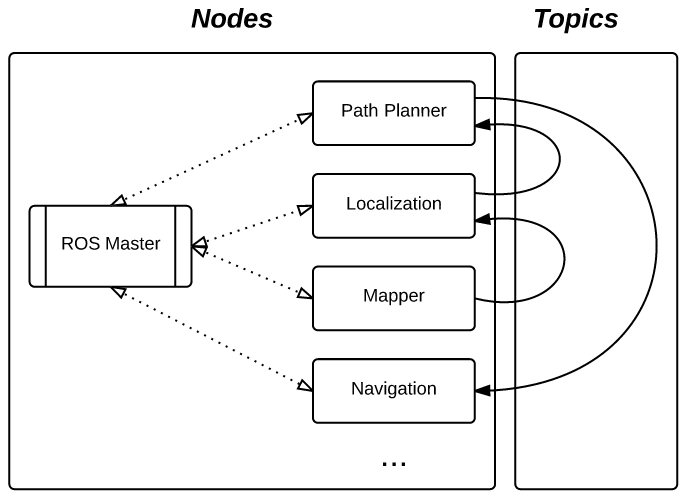
\includegraphics[width=\linewidth]{images/ros}
    \caption{Example of the Architecture of a ROS Network. Nodes are Linux processes which each handle independent tasks. Node communicate by publishing to and subscribing to channels called topics. The master node is a special node in charge of managing topics, publishers, and subscribers.}
    \label{fig:ros}
\end{figure}

In the context of the Robot Operating System, development of a database-backed message logging system is faced with several interesting challenges. First and foremost, the ROS publisher-subscriber network can potentially see data flows on the order of several gigabytes per minute when running a robot such as the PR2. Therefore, an important design decision for this utility would be to ensure the backend data store is capable of persisting large volumes of data in realtime. Additionally, robotics researchers often only have the computer running on the robot (server) and a separate desktop (client) in terms of hardware. Since robotics researchers often do not have a dedicated cluster for storing the data coming off of their robot, the backend data store for this utility needs to be able to provide this high-volume storage while only running on several machines (not a large cluster). Finally, much of the data to be stored consists of numerical values (joint angles, transpose vectors, audio packets, etc) and image-like data (laser scans, point clouds, stereo images, etc.), the data store needs to support rich querying interfaces which make it easy to analyze this type of data. With these considerations in mind, this work evaluates three potential database systems against three main criteria:

\begin{enumerate}
    \item What is the maximum throughput of each database under loads consisting of varying numbers of topics, sizes of messages, and frequency of messages? 
    \item Given a real world bag file dataset (specifically, the MIT Stata dataset), how well does the database perform (e.g. percent of messages persisted) when run in a single machine configuration?
    \item How rich is the query interface supported by the database, and how fast can typical robotics queries be executed? (e.g. ``Select all non-overlapping 1 minute intervals where the robot was in state $X$'', or ``Select all messages beginning 5 minutes before each system error was detected'')
\end{enumerate}

\section{Related Work}
Niemueller et al.~\cite{niemueller2012generic} developed an integration between ROS and MongoDB and benchmarked it. Our experiments use a version of their software, which we improved and modified for the purposes of running our own benchmarks. In their study, they showed that their system was comparable in performance to the native rosbag utility, with improved CPU and memory usage, and 30\% write throughput overhead. However, the paper did not attempt to find the maximum throughput supported by their system. Additionally, they did not compare the performance of their system to that of a relational database. Our work addresses both of these questions.

In a related approach, Dietrich et al.~\cite{dietrich2014ros} developed and benchmarked an integration between ROS and Cassandra, another popular NoSQL database. Their experiments found that their system outperformed a different ROS MongoDB system from the one described above, although the MongoDB system in question was only a data warehouse which stored messages as binary files and therefore had no querying capabilities. In this work, they also did not report the maximum throughput of their system, or do a comparison with relational databases. Importantly, the work of Dietrich et al. was founded on conclusions from a 2012 study by van der Veen et al. \cite{van2012sensor} indicating that Cassandra may be the best database (out of MongoDB, Cassandra, and PostgreSQL) for managing sensor network data. These conclusions in the van der Veen paper rely on a hardware setup of a server with 64 Gb of RAM and 22 CPU cores running their database. While this premise is sound for sensor network data collection, few roboticists have dedicated servers for robot data collection. A far more common setup in a robotics lab is a single external computer, plus the computer on board the robot. Given this stark difference in hardware, the van der Veen work does not appear to be a valid basis for robot data collection systems.

\section{Benchmark Studies}
In order to evaluate these three criteria, we conducted three studies comparing PostgreSQL, MongoDB, and SQLite3: 1) an initial throughput study, 2) a real-world dataset persistence performance study, and 3) a query timing study (corresponding to the three criteria laid out in section \ref{intro}).

\begin{figure}
    \centering
    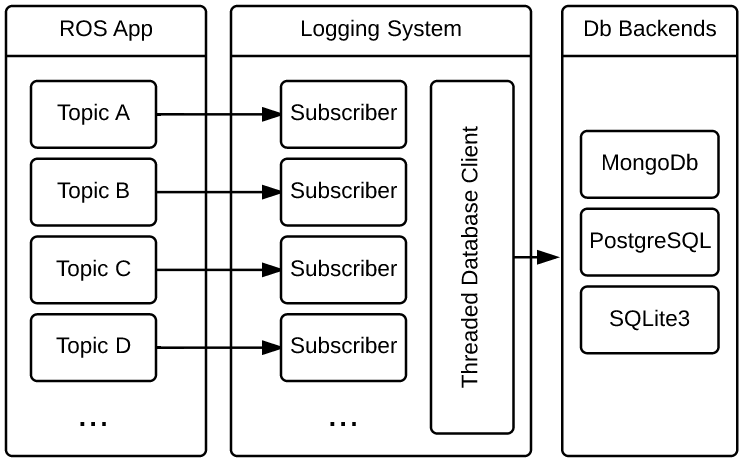
\includegraphics[width=\linewidth]{images/roslog}
    \caption{Design of the ROS Logging Test Framework. The logging system creates a thread for each topic in the current ROS network responsible for converting ROS messages to an equivalent JSON format. The subscriber threads pass prepared JSON messages to a database client responsible for persisting these JSON messages to a particular database.}
    \label{fig:roslog}
\end{figure}

\subsection{Systems and Datasets}
\label{sec:datasets}
In order to persist ROS messages, all messages were converted to a JSON (Javascript Object Notion) representation. The structure of JSON provides several benefits when it comes to storing ROS messages:
\begin{enumerate}
\item JSON allows for flexibility in message structure, thereby ensuring that changes in message structure, which are inevitable during the development of a robotics system, will not be breaking changes for the datastore,
\item JSON is structured in a very similar manner (nested dictionaries) to that of ROS messages allowing for simple conversion between the formats,
\item JSON can be queried against as opposed to traditional binary message representations.
\end{enumerate}

\begin{figure*}
    \centering
    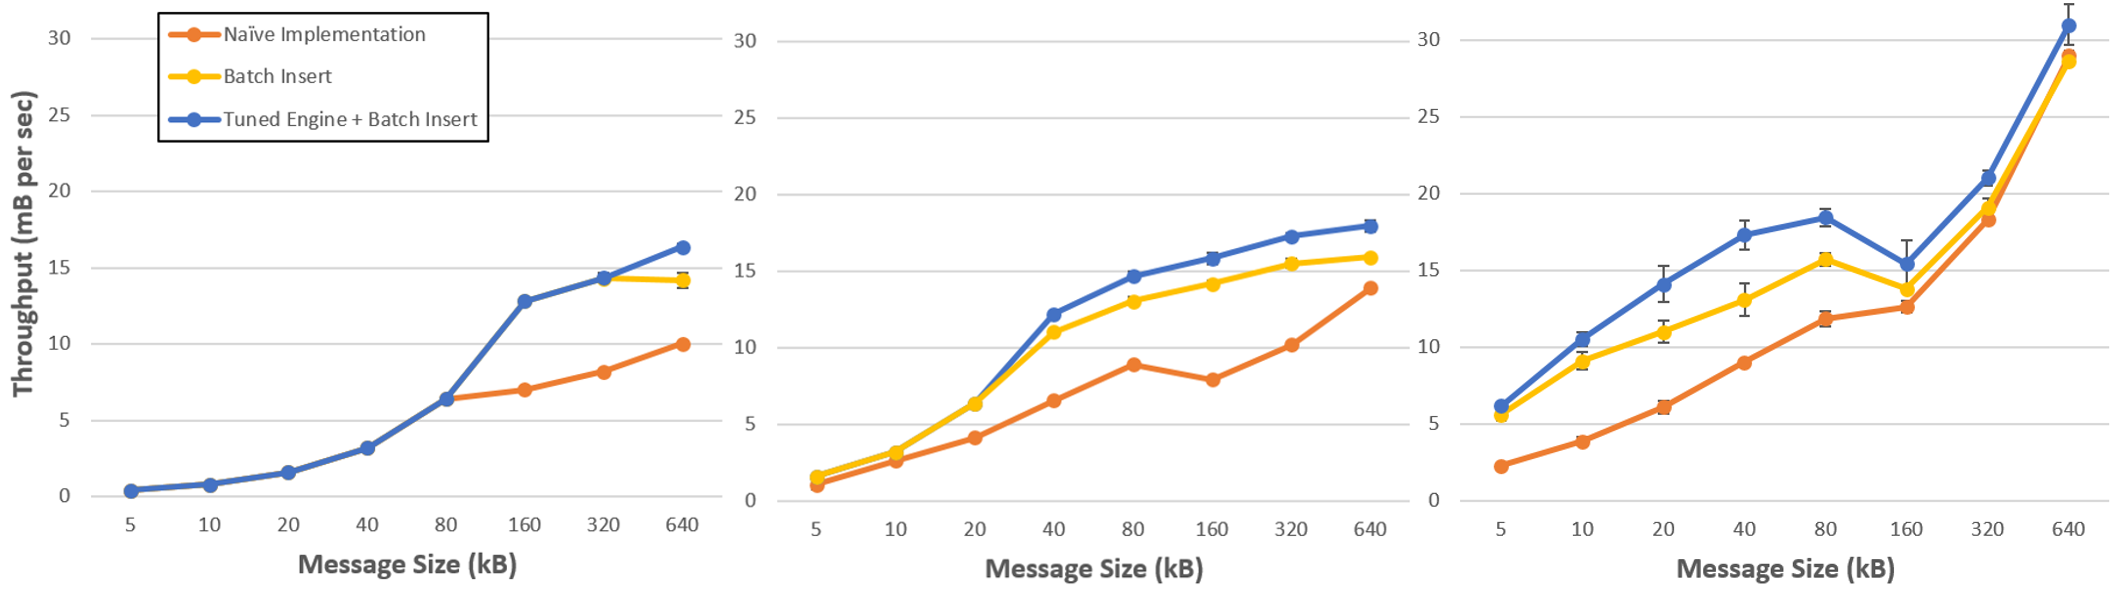
\includegraphics[width=\linewidth]{images/tuning}
    \subfloat[4 Messages Per Second]{%
        \hspace{0.3\linewidth}
        \label{4hz_tuning}%
    }
    \subfloat[16 Messages Per Second]{%
        \hspace{0.4\linewidth}
        \label{16hz_tuning}%
    }
    \subfloat[64 Messages Per Second]{%
        \hspace{0.3\linewidth}
        \label{64hz_tuning}%
    }
    \caption{Tuning PostgreSQL by Testing Throughput Across Multiple Frequencies and Message Sizes}
    \label{fig:tuning}
\end{figure*}

Given this choice of data representation, MongoDB was chosen as a good candidate database for evaluation since MongoDB is a NoSQL document-oriented database which stores all data in JSON and is optimized for fast JSON-based queries. While JSON has not traditionally been considered well suited to being stored in a relational database (having a potentially varied structure), recent advances in PostgreSQL 9.4 have added extensions which allow PostgreSQL to query against JSON data columns in a similar fashion to that of MongoDB, except through the high-level query language SQL. Therefore, PostgreSQL with JSON support was chosen as the second database to evaluate in this study. Finally, initial tests showed that the primary challenge in creating a ROS message logging database is that ROS can have potentially many messages streaming through its network at any given time (on the order of Gb per minute), making it challenging to persist all of the messages in the network as fast as they are generated. For this reason, SQLite3, an embedded database designed to have minimal overhead, was chosen as the third database to evaluate. While future work should be conducted to examine the potential of using streaming engines running on computer clusters for real-time analytics, this work focuses on the more common hardware setup for the average roboticist of a one to two computer system without the requisite resources for running extremely RAM intensive data stores such as the in-memory database VoltDb or the streaming engine Spark Streaming.

For the first criteria evaluated in this study (throughput), a synthetic dataset was generated by creating a message streaming ROS node with the ability to generate multiple topics running at the same frequency and sending messages of the same size in terms of bytes. To test the second criteria (real-world dataset performance), both a set of eight bag files obtained from previous research in our lab (referred to as the HCR dataset) and two bag files from the MIT Stata Center dataset were chosen \cite{fallon2013stata}. The MIT Stata Center data set encompasses a series of recordings of data from a PR2 robot driving around a building. It includes data types such as laser scans, accelerometer data, and images. While unconventional, these types of data are common in robotics research. Finally, in order to evaluate the third criteria (query performance), we populated databases with data from eight bag files from a dataset obtained from previous research, \textit{HCR}. The \textit{HCR} dataset consists of data recorded from a real-world user study, which was conducted prior to the work for this paper. In the study, users tried teleoperating a PR2 robot with a particular 3D user interface. The message types in this dataset include the locations of the 3D viewpoints the users used to look at the robot, the gripper state, and the gripper location, which are useful for testing queries against data reflecting a broad subset of possible message types in the ROS environment.

\begin{figure*}
    \centering
    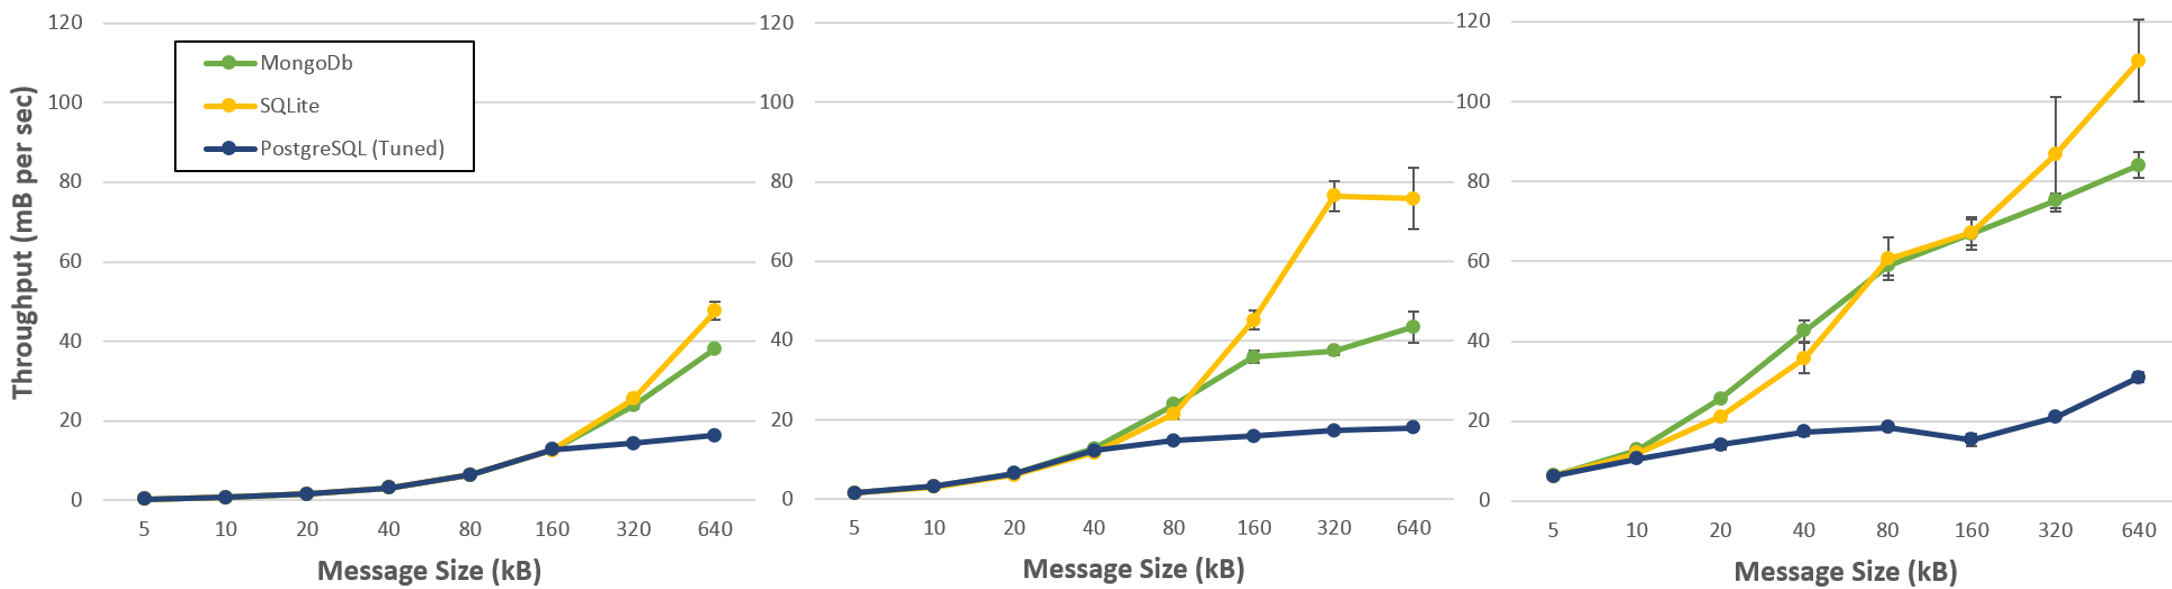
\includegraphics[width=\linewidth]{images/throughput}
    \subfloat[4 Messages Per Second]{%
        \hspace{0.3\linewidth}
        \label{4hz}%
    }
    \subfloat[16 Messages Per Second]{%
        \hspace{0.4\linewidth}
        \label{16hz}%
    }
    \subfloat[64 Messages Per Second]{%
        \hspace{0.3\linewidth}
        \label{64hz}%
    }
    \caption{Measurement of Throughput Across Multiple Frequencies and Message Sizes}
    \label{fig:throughput}
\end{figure*}

\subsection{Measuring Throughput}
\label{sec:throughput}
In the ROS ecosystem, published topics vary significantly in both the frequency at which messages are sent upon them, and in the size of messages belonging to the topic. This makes sense when considering that message types are very diverse, i.e. laser scans, joint angles, system events, etc. Therefore, in order to effectively compare the throughput of the three databases in consideration, several synthetic datasets were generated, reflecting potential types of messages that could appear in the ROS network. A constant 20 topics were generated for each synthetic data stream with each topic generating 500 messages. Additionally, each topic subscriber in the logging program was limited to an incoming message queue size of 10. This means that if messages are received by the logger faster than the underlying database can persist the messages, messages will be dropped from the incoming queue. This serves as a method of determining maximal throughput for each database. As frequencies and message sizes are increased, messages will begin to be dropped when the database has reached it maximum throughput for inserts corresponding to messages of the given size. Therefore, message sizes were varied on an exponential scale (each size is twice the previous message size) from 5000 bytes (approximately the size of a \textit{tf} message describing a coordinate frame transformation) to 0.64 Mb (approximately the size of a laser scan frame). To capture the effect of topic frequency on throughput, data streams were generated at three different frequencies: 4 hz, 16 hz, and 64 hz. Altogether, this resulted in the generation of 24 different data streams (3 frequencies by 8 message sizes). Each database was tested by logging each data stream 5 times in order to obtain reliable average throughput values over each stream. The experiment was run on a computer system running with an Intel Core i7-4770 CPU with 8 cores, 16 GB of memory, and a local hard disk.

\subsubsection{Tuning PostgreSQL}
\label{sec:tuning}
In preliminary tests of the throughput measurement procedure it was observed that PostgreSQL was performing significantly worse than both SQLite3 and MongoDB on the throughput experiment. It was determined that this was likely due to the fact that the our naive implementation of the PostgreSQL-ROS interface inserted each ROS message in autocommit mode. This means that each message was inserted in its own transaction. This clearly causes some amount of unnecessary overhead, although the degree to which using autocommit mode slows down PostgreSQL was unclear. Therefore, an additional test was run in which the naive PostgreSQL-ROS interface was re-engineered in order to allow message inserts to be batched into 2 second groups for each database transaction, under the hypothesis that this optimization could yield significantly greater throughput values by decreasing overhead. As can be seen in Figure \ref{fig:tuning}, this optimization did yield improved throughput for the PostgreSQL database. To further tune the PostgreSQL engine, both the effective cache size and shared buffer size were increased to rather aggressive levels (12Gb and 4Gb respectively) in order to encourage maximally efficient inserts. Again, this optimization improved overall PostgreSQL performance, but only by a small amount when considering the throughput values obtained by SQLite3 and MongoDB (see Figure \ref{fig:throughput}). Figure \ref{fig:throughput} references the throughput values for the final optimized version of the PostgreSQL engine determined in this section.

%; however, SQLite3 and MongoDB were still significantly better, often by factors of 2 to 3 times greater throughput.

\subsubsection{Results}
Results for the throughput evaluation against PostgreSQL (tuned as discussed in section \ref{sec:tuning}), MongoDB, and SQLite3 can be seen in Figure \ref{fig:throughput}. Figure \ref{fig:throughput} splits these results into three graphs, one for each of the frequency levels. Interestingly, PostgreSQL performed significantly worse than both SQLite3 and MongoDB. This is perhaps not particularly surprising seeing as how SQLite3 is designed to be an embedded database with minimal overhead, and MongoDB is specifically designed for handling JSON data whereas PostgreSQl is designed to manage relational data with extensions for JSON document data.

Figure \ref{fig:throughput} shows the throughput of each database system given a certain publishing rate and message size, for a fixed number of messages. The points on the left of each graph, where all three implementations achieved the same throughput, show that for small message sizes, all three implementations were able to persist all the messages we published. However, as the message sizes grow larger, we can see that only some fraction of the total number of messages generated were actually inserted into the database, indicating the maximal throughput for each database at these given message frequencies and sizes. 

As can be seen in Figure \ref{fig:throughput}, as message size and frequency increase, the observed maximal throughput increases. This is not surprising since increased message sizes enable each of the databases to perform writes of large blocks of data to the disk which are more efficient than writes of small amounts of data. Additionally, higher frequency ensures that the database is constantly working at storing messages, removing any idle periods that may have been present at lower frequencies.

\subsubsection{Logging System Design Implications}

These results lead to two design implications that should inform the development of future logging systems for ROS. First, in the case that only a single computer is available for logging, SQLite exhibits the best performance due to the fact that it has very low overhead and is therefore a good choice for database backends. Second, in contrast to the first design implication, SQLite is not designed to be distributed, therefore in the case that more than one machine is available for logging, MongoDB would be the best choice of database backends.

\subsection{Real World Performance}
\label{sec:realworld}
The previous section stress tested each of the databases by generating a fixed number of topics with messages of fixed sizes all sent at fixed frequencies. While this was a reasonable setup for measuring throughput, it is not necessarily representative of a real world work load. This is due to the fact that real world ROS networks contain many topics each with messages of different sizes and frequencies (see Figure \ref{fig:ros}). In order to evaluate how each of the databases performs on this type of real world dataset with significant variance among topics and messages, we tested the databases against several recordings from the MIT Stata Center dataset (labeled \textit{MIT1} and \textit{MIT2}). The MIT Stata Center dataset is a series of bagfiles consisting of recordings of image and laser data recorded at a high frequency by a robot exploring the Stata Center at MIT. This dataset is typically used for testing simultaneous localization and mapping algorithms and is therefore a set of recordings with very high rate of data flow. In order to test the real world performance of each database on a more moderate rate of data flow, several rosbag recordings obtained from the HCR dataset were also tested against (labeled \textit{HCR1} and \textit{HCR2}). This series of tests used the same logging framework as in Section \ref{sec:throughput} (described in Figure \ref{fig:roslog}).

\subsubsection{Results}
Figure \ref{fig:realworld} shows that for both \textit{HCR1} and \textit{HCR2}, all three databases successfully persisted 100\% of the messages. None of the databases were able to persist 100\% of messages for either of \textit{MIT1} or \textit{MIT2}. This is due to the fact that both MIT datasets contain high frequency recordings of large laser scans. While this issue of dropped messages could be resolved by storing the images and laser scans directly in a file system rather than in the database, this evaluation is interesting in that SQLite3 performed worst on each dataset whereas in the throughput evaluation, SQLite3 was found to have the highest throughput. This is likely an indication that SQLite3 performs best on homogeneous insert tasks (the synthesized messages in each run of the tests in section \ref{sec:throughput} were of the same size), but performs poorly when large amounts of non-homogeneous messages are inserted in the database. This allows us to draw the design implication that in a majority of cases, the best database to use for logging ROS messages in terms of data persistence is MongoDB.

\begin{figure}
    \centering
    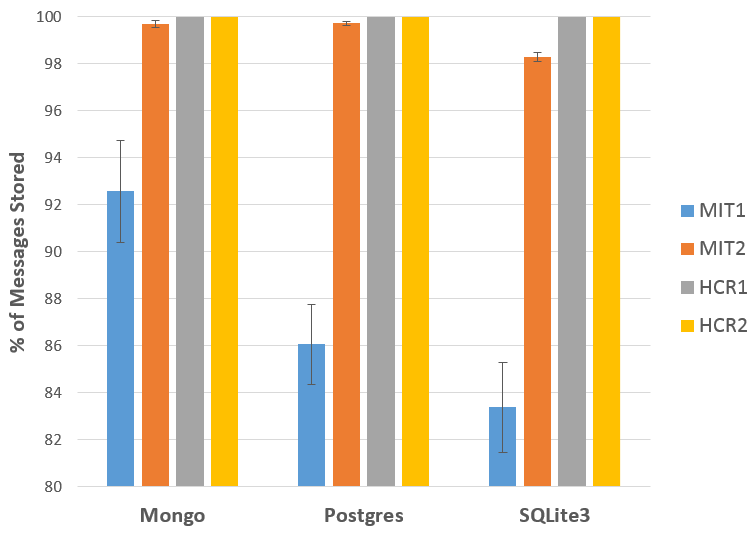
\includegraphics[width=\linewidth]{images/realworld}
    \caption{Percentage of Messages Persisted Across Four Real World Datasets. \textit{MIT1} and \textit{MIT2} are bagfiles from the MIT Stata center dataset and \textit{HCR1} and \textit{HCR2} are bagfiles from previous robotics experiments run in the Human-Centered Robotics Lab at the University of Washington. Note that the vertical axis shows the range (80, 100).}
    \label{fig:realworld}
\end{figure}

\subsection{Query Performance}
Up to this point, our work has been focused on efficiently and effectively persisting ROS messages to a database; however, we have yet to consider the flexibility and efficiency of querying against the databases after the ROS messages have been store. Therefore, in the last portion of our benchmarking study, we sought to evaluate the querying capabilities of PostgreSQL, SQLite3, and MongoDB in regards to queries that are potentially of interest to robotics researchers. To this end, we evaluated the time taken execute several representative queries against the \textit{HCR} dataset (see section \ref{sec:datasets}). The research questions we wanted to answer from the dataset are shown in Figure \ref{fig:hcrqueries}.

These queries were chosen to test a set of important capabilities for the logging system to have. Each system should have the ability to retrieve results and filter by a field inside the JSON message. Additionally, each system should efficiently support range queries. Finally, we wanted to see how well each system could compute a join, using the timestamp as a join key. Because messages are asynchronous, the join is on a small time range around one of the timestamps. The queries were also chosen to reflect questions that the researchers behind the \textit{HCR} dataset actually answered in their study, by manually processing the recordings.

\begin{figure}
\begin{enumerate}[label=Q\arabic*]
    \item Get the number of times the right gripper was closed
    \item Get the every viewpoint position when the viewpoint was behind the robot
    \item Get the number of times the right gripper was moved while in a particular region
    \item Get the number of times a grasp was attempted with the right gripper when the camera was in front of the robot (+/- 0.1 seconds)
\end{enumerate}
\caption{The queries we wanted to answer from the \textit{HCR} dataset.}
\label{fig:hcrqueries}
\end{figure}

\subsubsection{Results}

The time for each query is shown in table \ref{tab:queries}. See the appendix for the implementation of each query against each database. MongoDB performed the best across all queries, requiring less than 50 milliseconds for each of query 1, 2, and 3 and only about 250 milliseconds for query 4. Indexes on MongoDB designed to improve each query had minimal effect due to the fact that each query was already running very fast. PostgreSQL was the next fastest across all queries although it was an order of magnitude slower than MongoDB for each. This is clear evidence that PostgreSQL is designed as a relational database and is therefore not as highly optimized for JSON queries as MongoDB is. Interestingly, indexing PostgreSQL tables had no effect due to the fact that each query required casting string-typed JSON data to real values and PostgreSQL does not support creating JSON expression-based indexes that include casting operations. Finally, SQLite3 performed worst of all databases across all queries. This was caused by the fact that SQLite3 has no concept of a JSON datatype. Therefore, in order to run queries over JSON data, user-defined functions must be created for all operations required in each of the queries (e.g. the python function \textit{json\_eq\_field} was defined to evaluate the expression $json[`position.x`] > 0$). A consequence of the fact that user defined functions must be create to query against JSON data in a SQLite database is that all queries against the database necessarily require full sequential scans. This slows down the SQLite database significantly.

\begin{table}
    \centering
    \begin{tabular}{c | c | c | c | c}
        Database           & Q1     & Q2      & Q3      & Q4     \\
        \hline
        MongoDB            & <1     & 40      & 32      & 2.68e3 \\
        MongoDB (indexed)  & <1     & 12      & 44      & 668    \\
        Postgres           & 21.49  & 232.25  & 347.27  & 1.99e4 \\
        Postgres (indexed) & 1.14   & 225.45  & 352.11  & 1.95e4 \\
        SQLite3            & 1.20   & 2414.52 & 1547.70 & 4.85e5 
    \end{tabular}
    \caption{Query times, in milliseconds, for each query using MongoDB, PostgreSQL, and SQLite3. For MongoDB and PostgreSQL, we also report query times after creating indices designed for each query.}
    \label{tab:queries}
\end{table}

\section{Discussion}
The results from our three studies ultimately suggest that MongoDB would be the best database system to use for a ROS logging system. Although SQLite3 had higher throughput on the synthetic dataset, MongoDB had the highest throughput on a real world dataset. Additionally, MongoDB outperformed both PostgreSQL and SQLite3 in terms of query performance, especially on the query which required a join.

Using a database offers robotics researchers a convenient way to analyze their data. For example, it takes about 10 lines of Python code to manually process a bag file to find out how many times the right gripper was closed (Q1). But, using a database, the same query can be written with just a single line of SQL or Javascript. Our results showed that using MongoDB, queries could be completed in a couple of seconds or less, which is fast enough for researchers to interactively study their data.

On the other hand, some questions are easier to answer by hand writing code, as opposed to writing a query. For example, consider the problem of counting how many times the user changed the 3D viewpoint in the interface. The location of the 3D viewpoint is continuously published several times a second, so as the user changes their viewpoint in a single, fluid motion, each location will be logged with a slightly different position. Once the user stops moving the viewpoint, the location messages will be identical to each other. As a result, when there is a continuous run of distinct values for the viewpoint location, we say that the user is changing their viewpoint. Once the viewpoint locations stay the same, we say the user has stopped changing their viewpoint. In this case, writing a query would be far more difficult than writing code to process the data. 

This issue is an artifact of the type of data sent through ROS networks. Messages in ROS tend to reflect the state of a single sensor at a specific point in time. However, for analysis purposes, we are often interested in high-level changes in states. Additionally, because the messages are asynchronous, it is hard to join tuples based on time. For example, in Q4, we join the gripper position and the camera position using a time window of +/- 0.1 seconds.

\section{Future work}
One of the key issues that came up with PostgreSQL and SQLite3 throughout this study was that neither database system was designed to handle JSON structured data natively. This was especially noticeable when evaluating the database systems for query performance. One area that would be interesting to study is if we could trade throughput and flexiblity for query performance. For example, instead of storing ROS messages as JSON data, the logging system could transform ROS messages into flattened tuples of the appropriate type. This would allow the user to query the database without needing special JSON support. The user could also add indices on certain columns, which we were unable to do with PostgreSQL and SQLite in this study. One downside to this approach is that throughput would decrease, since easy message would have to be flattened out before inserting it into the database. However, as we saw earlier, PostgreSQL and SQLite3 had no problem inserting all the messages in the \textit{HCR} dataset. The other downside to this approach is that any change to the ROS message structure would require a schema change in the corresponding SQL tables. As a result, this solution would be best for small, one-off research projects.

Another area of future work is to analyze streaming data analysis solutions such as Apache Spark or VoltDB. These database systems could be useful for situations in which the robots are more established and are already deployed. These solutions would allow the developer to keep track of key statistics on the robot's sensor data in real-time.

\section{Conclusion}
In this paper, we characterized the performance of three different database systems for use in a robotics logging application. We compared their maximum throughput for both synthetic and real-world datasets. Finally, we evaluated their speed at conducting several queries that were drawn from previous robotics research. Overall, we found that MongoDB would be the best database system to back a logging application, both because it had good throughput, and because its data model enabled fast queries across the datasets.

\bibliographystyle{abbrv}
\bibliography{references.bib}  

\clearpage

\onecolumn

\appendix
\vspace{0.5cm}

\section{MongoDB Queries (\textit{in JavaScript})}
\vspace{0.5cm}
\begin{lstlisting}[style=htmlcssjs]
var c = db.r_gripper_controller__command.find({'position': 0.0}).count();

var c = db.rviz_camera_publisher__camera_pose.find({'position.x': {$lte: 0}}).count();

var c = db.r_cart__command_pose.find({
  'pose.position.z': {$gt: 1},
  'pose.position.y': {$gt: -0.5, $lt: 0.5},
  'pose.position.x': {$gt: 0.5, $lt: 1}
}).count();

var c = db.r_gripper_controller__command.find({'position': 0.0}).map(
  function(evt) {
    var evtTime = evt._meta.inserted_at.getTime();
    var row = db.rviz_camera_publisher__camera_pose.findOne({
      'position.x': {$gte: 0},
      '_meta.inserted_at': {
        $lt: new Date(evtTime + 500),
        $gt: new Date(evtTime - 500)
      }
    })
    return row;
  }
).length;

db.r_gripper_controller__command
  .createIndex({"position": 1});
  
db.rviz_camera_publisher__camera_pose
  .createIndex({"position.x": 1, "_meta.inserted_at": 1});
  
db.r_cart__command_pose
  .createIndex({"pose.position.x": 1, "pose.position.y": 1, "pose.position.z": 1});
\end{lstlisting}


\section{PostgreSQL Queries (\textit{in SQL})}
\vspace{0.5cm}

\begin{lstlisting}[style=sql]
SELECT 	COUNT(*) 
FROM 	r_gripper_controller__command 
WHERE 	(data->>'position')::REAL = 0;

SELECT	COUNT(*)
FROM	rviz_camera_publisher__camera_pose
WHERE	(data->'position'->>'x')::REAL <= 0;

SELECT	COUNT(*)
FROM    r_cart__command_pose    --Contains right gripper location info
WHERE   (data->'pose'->'position'->>'z')::REAL > 1
AND     (data->'pose'->'position'->>'y')::REAL > -0.5
AND     (data->'pose'->'position'->>'y')::REAL < 0.5
AND     (data->'pose'->'position'->>'x')::REAL > 0.5
AND     (data->'pose'->'position'->>'x')::REAL < 1;

SELECT	COUNT(*)
FROM	r_gripper_controller__command a
WHERE	(data->>'position')::REAL = 0
AND     EXISTS (
            SELECT  *
            FROM    rviz_camera_publisher__camera_pose b
            WHERE   ABS(EXTRACT(EPOCH FROM 
                        CAST(a.data->'_meta'->>'inserted_at' AS TIMESTAMP WITH TIME ZONE) - 
                        CAST(b.data->'_meta'->>'inserted_at' AS TIMESTAMP WITH TIME ZONE)
                    )) < 0.5
            AND     (b.data->'position'->>'x')::REAL >= 0
        );
\end{lstlisting}

\section{SQLite3 Queries (\textit{in Python})}
\vspace{0.5cm}

\begin{lstlisting}[style=pystyle]
# Example UDF to test a JSON field for equality against a constant
def get_val(self, doc, key):
		d = json.loads(doc)

		val = pq(d, key)

		return val

def json_eq_field(self, doc, key, value):
	val = self.get_val(doc, key)

	if val is None:
		return False

	return val == value
	
#Queries
lite = NSQlite3('querytestlarge.db', JSONAdapter())
coll = lite.collection()

#Q1
sql = '''SELECT COUNT(*) as count
		 FROM   r_gripper_controller__command 
		 WHERE  json_eq_field(msg, ?, ?);'''

coll.execute(sql, ['position', 0]).all()

#Q2
sql = '''SELECT COUNT(*) 
		 FROM   rviz_camera_publisher__camera_pose
		 WHERE  json_le_field(msg, ?, ?);'''

coll.execute(sql, ['position.x', 0]).all()

#Q3
sql = '''SELECT COUNT(*) 
		 FROM   r_cart__command_pose
		 WHERE  json_gt_field(msg, ?, ?)
		 AND    json_gt_field(msg, ?, ?)
		 AND    json_lt_field(msg, ?, ?)
		 AND    json_gt_field(msg, ?, ?)
		 AND    json_lt_field(msg, ?, ?);'''
		 
vals = ['pose.position.z', 1, 
		'pose.position.y', -0.5, 
		'pose.position.y', 0.5, 
		'pose.position.x', 0.5, 
		'pose.position.x', 1]
		
coll.execute(sql, vals).all()

#Q4
sql = '''SELECT COUNT(*)
		 FROM 	r_gripper_controller__command a
		 WHERE 	json_eq_field(a.msg, ?, ?)
		 AND   	EXISTS (
		 			SELECT 	*
		 			FROM 	rviz_camera_publisher__camera_pose b
		 			WHERE 	json_get_time_diff(a.msg, ?, b.msg, ?) < 500
		 			AND   	json_ge_field(b.msg, ?, ?)
		 	   	);'''

vals = ['position', 0.0, 
		'_meta.inserted_at', 
		'_meta.inserted_at',
		'position.x', 0]

coll.execute(sql, vals).all()
\end{lstlisting}

\balancecolumns

\end{document}

